\documentclass{article}

\usepackage[utf8]{inputenc}
\usepackage[a4paper, total={6.3in, 8.8in}]{geometry}
\usepackage{amsmath}
\usepackage{bm}
\usepackage{amsfonts}
\usepackage{graphicx}
\usepackage{amssymb}  % assumes amsmath package installed
\usepackage{graphics} % for pdf, bitmapped graphics files
\usepackage{caption}
\usepackage{subcaption}
\usepackage{todonotes}
\usepackage{titling}
\usepackage{float}
\newcommand{\subtitle}[1]{%
  \posttitle{%
    \par\end{center}
    \begin{center}\large#1\end{center}
    \vskip0.5em}%
}

\title{Exercise Session 3: Unsupervised Learning and Large Scale Problems}
\subtitle{\Large{Support Vector Machines Report - Final Report}}
\author{Victor van Wymeersch - R0690930}
\date{May 2022}

\begin{document}

\maketitle
    
\section{Exercises}
    \subsection{Kernel principle component analysis} 
        % KPCA
        \begin{figure}[h]
             \centering
             \hspace{0.05\textwidth}
             % linear
             \begin{subfigure}[b]{0.4\textwidth}
                 \includegraphics[width=\textwidth]{Assignment 3/figures/1_1/linear_kpca.pdf}
                 \caption{Linear PCA}
                 \label{fig:linear_pca}
             \end{subfigure}
             \hfill
            % KPCA
             \begin{subfigure}[b]{0.4\textwidth}
                 \includegraphics[width=\textwidth]{Assignment 3/figures/1_1/kpca_nc_4_method_lanczos_sig2_0.4.pdf}
                 \caption{KPCA}
                 \label{fig:nonlinear_KPCA}
             \end{subfigure}
             \hspace{0.05\textwidth}
            \caption{Unsupervised regression using Linear PCA (a) and K-PCA (b).}
        \end{figure}
        
    \subsection{Spectral clustering} 
        % Spectral clustering results 
        \begin{figure}[h]
             \centering
             \begin{subfigure}[b]{0.3\textwidth}
                 \includegraphics[width=\textwidth]{Assignment 3/figures/1_2/spectral_rings_data.pdf}
                 \caption{Two spectral rings}
                 \label{fig:spectral_1}
             \end{subfigure}
             \hfill
             \begin{subfigure}[b]{0.3\textwidth}
                 \includegraphics[width=\textwidth]{Assignment 3/figures/1_2/spectral_rings_sig2_0.005.pdf}
                 \caption{$\sigma^2 = 0.005$}
                 \label{fig:spectral_2}
             \end{subfigure}
            \hfill
             \begin{subfigure}[b]{0.3\textwidth}
                 \includegraphics[width=\textwidth]{Assignment 3/figures/1_2/spectral_rings_sig2_0.010.pdf}
                 \caption{$\sigma^2 = 0.005$}
                 \label{fig:spectral_3}
             \end{subfigure}
                         \hfill
             \begin{subfigure}[b]{0.3\textwidth}
                 \includegraphics[width=\textwidth]{Assignment 3/figures/1_2/spectral_rings_sig2_0.020.pdf}
                 \caption{$\sigma^2 = 0.020$}
                 \label{fig:spectral_4}
             \end{subfigure}
            \hfill
             \begin{subfigure}[b]{0.3\textwidth}
                 \includegraphics[width=\textwidth]{Assignment 3/figures/1_2/spectral_rings_sig2_0.050.pdf}
                 \caption{$\sigma^2 = 0.050$}
                 \label{fig:spectral_5}
             \end{subfigure}
                         \hfill
             \begin{subfigure}[b]{0.3\textwidth}
                 \includegraphics[width=\textwidth]{Assignment 3/figures/1_2/spectral_rings_sig2_0.100.pdf}
                 \caption{$\sigma^2 = 0.100$}
                 \label{fig:spectral_6}
             \end{subfigure}
            \caption{Spectral clustering results on Two Rings dataset for different values of $\sigma^2$.}
        \end{figure}
    
    \subsection{Fixed-size LS-SVM}
        % Fixed-size LS-SVM 
        \begin{figure}[h]
             \centering
             \begin{subfigure}[b]{0.3\textwidth}
                 \centering
                 \includegraphics[width=\textwidth]{Assignment 3/figures/1_3/subsets_sig2_0.001.pdf}
                 \caption{$\sigma^2 = 0.001$}
                 \label{fig:subsets_sigma_1}
             \end{subfigure}
            \hfill
             \begin{subfigure}[b]{0.3\textwidth}
                 \centering
                 \includegraphics[width=\textwidth]{Assignment 3/figures/1_3/subsets_sig2_0.100.pdf}
                 \caption{$\sigma^2 = 0.050$}
                 \label{fig:subsets_sigma_2}
             \end{subfigure}
             \hfill
             \begin{subfigure}[b]{0.3\textwidth}
                 \centering
                 \includegraphics[width=\textwidth]{Assignment 3/figures/1_3/subsets_sig2_1000.000.pdf}
                 \caption{$\sigma^2 = 1000$}
                 \label{fig:subsets_sigma_3}
             \end{subfigure}
            \caption{Fixed-size LS-SVM subset of datapoints for varying values of $\sigma^2$.}
        \end{figure}
        
        
        % Fixed size vs L0 approximation 
        \begin{figure}[h]
             \centering
             \begin{subfigure}[b]{0.3\textwidth}
                 \centering
                 \includegraphics[width=\textwidth]{Assignment 3/figures/1_3/time.png}
                 \caption{Computation time}
                 \label{fig:l0computation_time}
             \end{subfigure}
            \hfill
             \begin{subfigure}[b]{0.3\textwidth}
                 \centering
                 \includegraphics[width=\textwidth]{Assignment 3/figures/1_3/error.png}
                 \caption{Error}
                 \label{fig:l0error}
             \end{subfigure}
             \hfill
             \begin{subfigure}[b]{0.3\textwidth}
                 \centering
                 \includegraphics[width=\textwidth]{Assignment 3/figures/1_3/sv.png}
                 \caption{Number of support vectors}
                 \label{fig:l0Number_supports}
             \end{subfigure}
            \caption{Fixed-size LS-SVM vs $L_0$ norm SVM results in terms of computation time (a), errors (b), and number of support vectors (c).}
        \end{figure}
        
\section{Homework Problems} 

    \subsection{Kernel principle component analysis}
        % Reconstruction for different sigma2 values 
        \begin{figure}[h]
             \centering
             \begin{subfigure}[b]{0.3\textwidth}
                 \centering
                 \includegraphics[width=\textwidth]{Assignment 3/figures/2_1/KPCA_sigmafactor_1.00.pdf}
                 \caption{$\sigma^2 = 1$}
                 \label{fig:kpca_digits_1}
             \end{subfigure}
            \hfill
             \begin{subfigure}[b]{0.3\textwidth}
                 \centering
                 \includegraphics[width=\textwidth]{Assignment 3/figures/2_1/KPCA_sigmafactor_10.00.pdf}
                 \caption{$\sigma^2 = 10$}
                 \label{fig:kpca_digits_2}
             \end{subfigure}
             \hfill
             \begin{subfigure}[b]{0.3\textwidth}
                 \centering
                 \includegraphics[width=\textwidth]{Assignment 3/figures/2_1/KPCA_sigmafactor_100.00.pdf}
                 \caption{$\sigma^2 = 100$}
                 \label{fig:kpca_digits_3}
             \end{subfigure}
            \caption{KPCA denoising results for different values of $\sigma^2$ using a RBF kernel.}
        \end{figure}
        
        % Linear vs RBF KPCA for large noise factor 
        \begin{figure}[h]
             \centering
             % KPCA
             \begin{subfigure}[b]{0.3\textwidth}
                 \centering
                 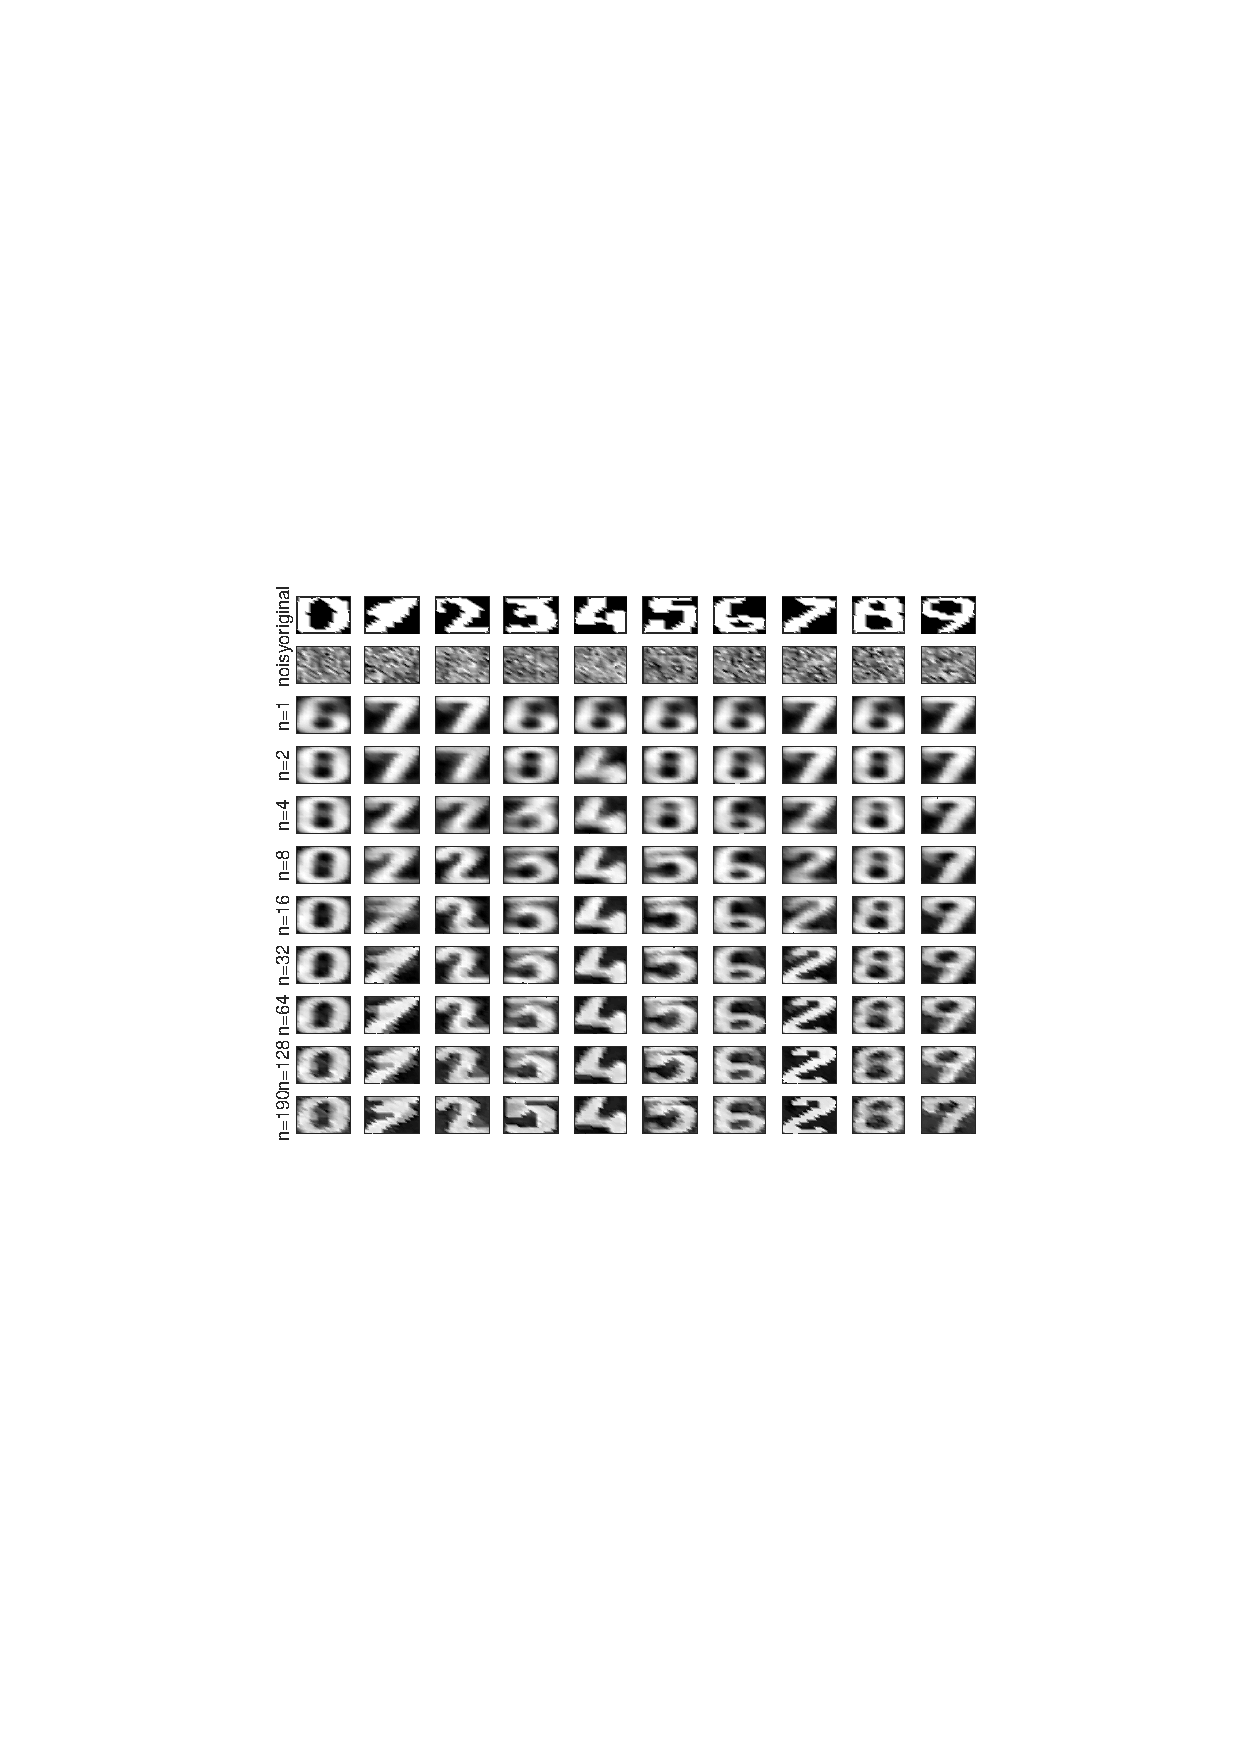
\includegraphics[width=\textwidth]{Assignment 3/figures/2_1/KPCA.pdf}
                 \caption{KPCA}
                 \label{fig:kpca}
             \end{subfigure}
            \hfill
            % Linear pca
             \begin{subfigure}[b]{0.3\textwidth}
                 \centering
                 \includegraphics[width=\textwidth]{Assignment 3/figures/2_1/Linear_PCA.pdf}
                 \caption{Linear PCA}
                 \label{fig:lin_pca}
             \end{subfigure}
            \caption{Result of KPCA (a) and Linear PCA denoising (b) of handwritten digits with a noise factor of 1.0}
        \end{figure}
    
        
    \subsection{Fixed-size LS-SVM}
    
    
        \subsubsection{Shuttle (statlog)}
            
            \begin{figure}[h]
             \centering
             \begin{subfigure}[b]{0.3\textwidth}
                 \centering
                 \includegraphics[width=\textwidth]{Assignment 3/figures/1_3/computation_time_comparison.pdf}
                 \caption{Computation time}
                 \label{fig:l0computation_time}
             \end{subfigure}
            \hfill
             \begin{subfigure}[b]{0.3\textwidth}
                 \centering 
                 \includegraphics[width=\textwidth]{Assignment 3/figures/1_3/error_comparison.pdf}
                 \caption{Error}
                 \label{fig:l0error}
             \end{subfigure}
             \hfill
             \begin{subfigure}[b]{0.3\textwidth}
                 \centering
                 \includegraphics[width=\textwidth]{Assignment 3/figures/1_3/Number_of_support_vectors.pdf}
                 \caption{$\sigma^2 = 1000$}
                 \label{fig:l0Number_supports}
             \end{subfigure}
            \caption{Fixed-size LS-SVM vs $L_0$ norm SVM results in terms of computation time (a), errors (b), and number of support vectors (c).}
        \end{figure}
        
        
        
        \subsubsection{California}
        
            \begin{figure}[h]
             \centering
             \begin{subfigure}[b]{0.3\textwidth}
                 \centering
                 \includegraphics[width=\textwidth]{Assignment 3/figures/1_3/computation_time_comparison.pdf}
                 \caption{Computation time}
                 \label{fig:l0computation_time}
             \end{subfigure}
            \hfill
             \begin{subfigure}[b]{0.3\textwidth}
                 \centering
                 \includegraphics[width=\textwidth]{Assignment 3/figures/1_3/error_comparison.pdf}
                 \caption{Error}
                 \label{fig:l0error}
             \end{subfigure}
             \hfill
             \begin{subfigure}[b]{0.3\textwidth}
                 \centering
                 \includegraphics[width=\textwidth]{Assignment 3/figures/1_3/Number_of_support_vectors.pdf}
                 \caption{$\sigma^2 = 1000$}
                 \label{fig:l0Number_supports}
             \end{subfigure}
            \caption{Fixed-size LS-SVM vs $L_0$ norm SVM results in terms of computation time (a), errors (b), and number of support vectors (c).}
        \end{figure}
\end{document}
